\clearpage
\phantomsection

\setcounter{chapter}{1}
\chapter[{ĐÁNH GIÁ ẢNH HƯỞNG CỦA CẤU HÌNH MẢNG ĂNG-TEN TRONG NHẬN DẠNG HỆ THỐNG MIMO KÍCH THƯỚC LỚN}]{Đánh giá ảnh hưởng của cấu hình mảng ăng-ten trong nhận dạng hệ thống MIMO kích thước lớn}
\label{sec:CRB}

Trong chương này, tác giả sẽ xem xét sự ảnh hưởng của các cấu hình mảng ăng-ten khác nhau đến sai số của việc ước lượng kênh truyền trong các hệ thống mMIMO. Đầu tiên, mô hình kênh truyền có cấu trúc và kiến trúc của hai mảng ăng-ten gồm 1D và 3D sẽ được trình bày. Sau đó là sơ lược về việc sử dụng đường CRB để ước lượng sai số trong các bộ nhận dạng sử dụng pilot và SB. Các kết quả mô phỏng được đưa ra để cho thấy hiệu quả của mô hình kênh truyền có cấu trúc, mảng ăng-ten 3D (UCyA), và phương pháp ước lượng SB trong việc nhận dạng hệ thống viễn thông.
% \section{Introduction}\label{Intro}
% Massive MIMO (Multiple-Input Multiple-Output) is a technology in 5G wireless communications that uses a large number of antennas at the base station to communicate simultaneously with multiple user devices in the same frequency band. Massive MIMO combined with Orthogonal Frequency Division Multiplexing (OFDM) obtains the numerous benefits of coverage, capacity, spectral and energy efficiency~\cite{Elhoushy2022}. 

% In communications, to recover source signals exactly, systems must get the channel state information (CSI). The known training symbols, called pilots, are embedded in the data to estimate CSI and synchronization. The length of pilot sequence should be larger than the number of elements in the antenna array. Because of the huge number of antenna elements, channel estimation in massive MIMO systems is very complex with a long training overhead~\cite{Liang2019}.

% There are two popular wireless channel models that are unstructured and structured models. The unstructured model is used mostly because of simplicity but it is not really suitable for millimeter wave with several significant reflective waves. This paper relates to semi-blind channel estimation in millimeter wave MIMO-OFDM systems. Semi-blind (SB) channel estimation algorithms are the combination of conventional training based methods and blind methods. They use several pilot symbols and other kinds of information~\cite{abed1997}. SB algorithms can reduce the number of pilot symbols efficiently but maintain acceptable accuracy~\cite{Rekik2021}. In the unstructured channel model, paths between each pair of transmitter and receiver antenna are described as complex gains~\cite{Swindlehurst2022} while the structured model includes complex gains, Directions of Departure (DoD) and Directions of Arrival (DoA). This model is also called specular or geometric channel model~\cite{Ladaycia2017, Swindlehurst2022}.

%  In~\cite{POORMOHAMMAD2017}, Poormohammad \textit{et al.} proposed that the geometries of antenna arrays certainly affect the accuracy of the DoA and DoD estimation. Furthermore, when the number of antennas becomes larger, 3D antenna arrays save significant installation space compared to 1D- and 2D arrays. Generally, most studies in the literature only consider a system of 1D or 2D antenna arrays. Thereby, in this work, we analysis of the performance bound of the semi-blind channel estimation in 3D-massive MIMO array geometries. For the SB method, besides the pilots part, the data symbols are assumed to be i.i.d and known statistical. The performances of systems are measured by Cramér Rao  Bound (CRB)~\cite{Ladaycia2017} for two antenna array structures, i.e., Uniform Linear Array (ULA) and Uniform Cylindrical Array (UCyA). From the simulation results, the UCyA outperforms the traditional ULA array regarding SNR and the number of elements in arrays.
 
% Our contribution in this paper is to propose a CRB derivation for SB channel estimation UCyA structure. The specular model of 3D-massive MIMO is presented in section 2. CRB deviations for training and SB channel estimation method in unstructured and specular models are shown in section 3. At last, the performance of ULA and UCyA structures are compared in numerical experiments.

\section{Mô hình kênh truyền có cấu trúc}\label{SM}

Trong chương này, mô hình toán của một hệ thống mMIMO sử dụng điều chế ghép kênh phân chia theo tần số trực giao (OFDM - Orthogonal frequency-division multiplexing) với $K$ sub-carriers trong kênh đường lên vẫn gồm $T$ ăng-ten (mono-antenna) phát, và $L$ ăng-ten thu. Mỗi ký hiệu OFDM bao gồm $K$ ký hiệu dữ liệu và một phần tiền tố vòng (CP - Cyclic Prefix). Giả sử độ dài của CP lớn hơn hoặc bằng thời gian trễ tối đa của kênh truyền (coherent time). Tại ăng-ten thu thứ $l$, sau khi đã loại bỏ thành phần CP và thực hiện biến đổi Fourier (FFT - Fast fourier transform), tín hiệu đầu ra $\mathbf{x}_l$ được biểu diễn như sau~\cite{Ladaycia2017}

% This paper considers a massive MIMO-OFDM communication system in the Uplink channel with $N_t$ transmit mono-antennas and $N_r$ receive antennas with $K$ sub-carriers. 
% Suppose that, the mmWave MIMO channels are models in terms of channel filter taps ($L$)~\cite{tse}. 
% Each OFDM symbol consists of $K$ data symbols and a CP (Cyclic Prefix) to avoid inter-symbol interference. Such that the length of CP must be equal to or greater than the maximum channel delay (coherent time). At $r$-th receive antenna, after removing Cyclic Prefix and then FFT $K$-point of OFDM data samples, the output signal $\boldsymbol{y}_{r}$ in time~domain can be expressed by~\cite{Ladaycia2017}:

% \begin{equation}
%     \boldsymbol{y}_{r} = \tilde{\mathbf{X}}\mathbf{h} +\boldsymbol{v}_r
% \end{equation}

\begin{equation}
    \mathbf{x}_{l}=\sum_{t=0}^{T-1} \mathcal{F} \mathcal{T}\left(h_{l, t}\right) \frac{\mathcal{F}}{K} \mathbf{s}_{k}+\mathbf{w}_{l}
\end{equation}
trong đó $\mathcal{F}$ đại diện cho ma trận Fourier rời rạc, gồm $K$ điểm và $\mathcal{T}$ là ma trận lặp lại của $h_{l, t}$. Tiếp đến $\mathbf{s}_{k}$ là ký hiệu OFDM thứ $k$ có độ dài $K$ và $\mathbf{w}_{l} \in \mathbb{C}^{L \times 1}$ là tạp âm AWGN có dạng i.i.d phân bố Gaussian $\mathcal{C} \mathcal{N}\left(\mathbf{0}, \sigma_{\mathbf{w}}^{2} \mathbf{I}_L\right)$, $\mathbb{E}\left\{\mathbf{w}_{l} \mathbf{w}_{l}^{\top}\right\}=\mathbf{0}$. 
% In the unstructured channel model, $\mathbf{h}_{r, j}$ of order $L-1$ is the channel impulse response in a period of time between $j$-th transmitter and $r$-th receiver. 
Cuối cùng, $h_{l, t}$ là thành phần thuộc ma trận kênh truyền được biểu diễn dưới dạng véc-tơ $\mathbf{h} \in \mathbb{C}^{L T \times 1}$.
\begin{equation}
    \label{eq:1}
    \begin{aligned} 
        \mathbf{h} &=\left[\mathbf{h}_{0}^{\top}, \mathbf{h}_{1}^{\top}, \ldots, \mathbf{h}_{L - 1 }^{\top}\right]^{\top}, \\ \mathbf{h}_{l} &=\left[h_{l, 0}, h_{l, 1}, \ldots, h_{l, T - 1 }\right]^{\top}
    \end{aligned}
\end{equation}
với $(.)^\top$ là phép chuyển vị (transpose) ma trận. Giả sử rằng $M$ là số lượng đường truyền giữa một cặp ăng-ten phát, thu. Dựa trên hướng tiếp cận mô hình kênh truyền có cấu trúc (stuctured), tác giả mô hình $h_{l, t}$ tương ứng với $M$ đường truyền, mỗi đường truyền bao gồm hệ số khuếch đại phức (complex gain) và véc-tơ lái ($\varphi$ - steering) như sau

% Assume that $L$ is the number of paths between a transmit antenna and receiver. Following the specular channel approach, we model the $\mathbf{h}_{r, j}$ according to $L$ paths, complex path gains, and steering vectors, as follows:

\begin{equation}
\label{eq:2}
    % \begin{aligned}
        h_{l, t} = \sum\limits_{m=0}^{M-1} \beta_{m, t} e^{\varphi_{m, t}} = \sum\limits_{m=0}^{M-1} \beta_{m, t} \cdot e^{-i k_s c(\theta_{m, t}, \phi_{m, t})} 
    % \end{aligned}
\end{equation}
% where $l= 0,1,\ldots, L-1$. 
% where $N, M_n$ are the number of clusters and the number of rays within each cluster, respectively. 
với mỗi đường truyền thứ $m$, hệ số $\beta$ biểu diễn cho hệ số khuếch đại phức. Góc ngẩng (zenith) và góc phương vị (azimuth) của hướng sóng đến (DoA)\footnote{Để đơn giản hoá, thông tin về hướng sóng phát (DoD - Direction of departure) được coi là không biết trước tại bên thu của kênh đường lên.} lần lượt là  $\theta$, $\phi$. Ký hiệu $(\cdot)$ tương ứng là phép nhân vô hướng.
% for the $l$-th ray, $\beta$ represents complex path gain.
% Zenith and azimuth angle of DoA\footnote{For simplicity, we supposed that the DoD (Direction of Departure) information is not available in the receivers.} are $\theta$, $\phi$, respectively. The $(\cdot)$ being scalar product. 
% The magnitude of $\mathbf{h}_{r, j}$ depends on path loss, as function of $f_c$ (carrier frequency), $d$ (distance), given by:
% \begin{equation}
%     \begin{aligned}
%         \alpha_{n, m, j}(f_c, d)[\mathrm{dB}]=& \mathrm{FSPL}\left(f_c, d_{0}\right)+10 n \log _{10}\left(\frac{d}{d_{0}}\right)+\chi_{\sigma}, \\
%         & \text { for } d \geq d_{0}, \text { where } d_{0}=1\mathrm{m}
%     \end{aligned}
% \end{equation}
% with $\operatorname{FSPL}\left(f_c, d_{0}\right)=20 \log _{10}\left(4 \pi d_{0} c / f_c\right)$, where $c$ is the speed of light, $n$ denotes the path loss exponent (PLE), and $\chi_{\sigma}$ is the shadow fading which is modeled as a lognormal
% random variable with zero mean and $\sigma$ standard deviation.
Các ký hiệu còn lại trong phương trình~(\ref{eq:2}) lần lượt là
\begin{equation}
    \begin{aligned}
        &k_s = 2\pi/\lambda \\
        &c(\theta_{m, t}, \phi_{m, t}) = \widehat{\boldsymbol{c}} \cdot \boldsymbol{c}_p \\
        &\widehat{\boldsymbol{c}}=\sin \theta_{m, t} \cos \phi_{m, t} \widehat{\boldsymbol{x}}+\sin \theta_{m, t} \sin \phi_{m, t} \widehat{\boldsymbol{y}}+\cos \theta_{m, t} \widehat{\boldsymbol{z}} \\
        &\boldsymbol{c}_p=x_{p} \widehat{\boldsymbol{x}}+y_{p} \widehat{\boldsymbol{y}}+z_{p} \hat{\boldsymbol{z}}
    \end{aligned}
\end{equation}
trong đó, $\lambda$ là bước sóng; $\widehat{\boldsymbol{c}}$ là véc-tơ đơn vị trong hệ toạ độ đề-các (Descartes) ba chiều của các véc-tơ DoA; và $\boldsymbol{c}_p$ là vị trí của phần tử thứ $p$ trong mảng ăng-ten bên thu ứng với toạ độ ($x_p, y_p, z_p$).
% where $\lambda$ is the wavelength; $\widehat{\boldsymbol{s}}$ is the unit vector in the direction of the field point; $\boldsymbol{s}_p$ is the position of $p$-th element in receiver's antenna array ($x_p, y_p, z_p$).
\begin{figure}[ht]
    \centering
    \subcaptionbox{Mảng thẳng cách đều (ULA - Uniform Linear Array)}
        [0.49\linewidth]
        {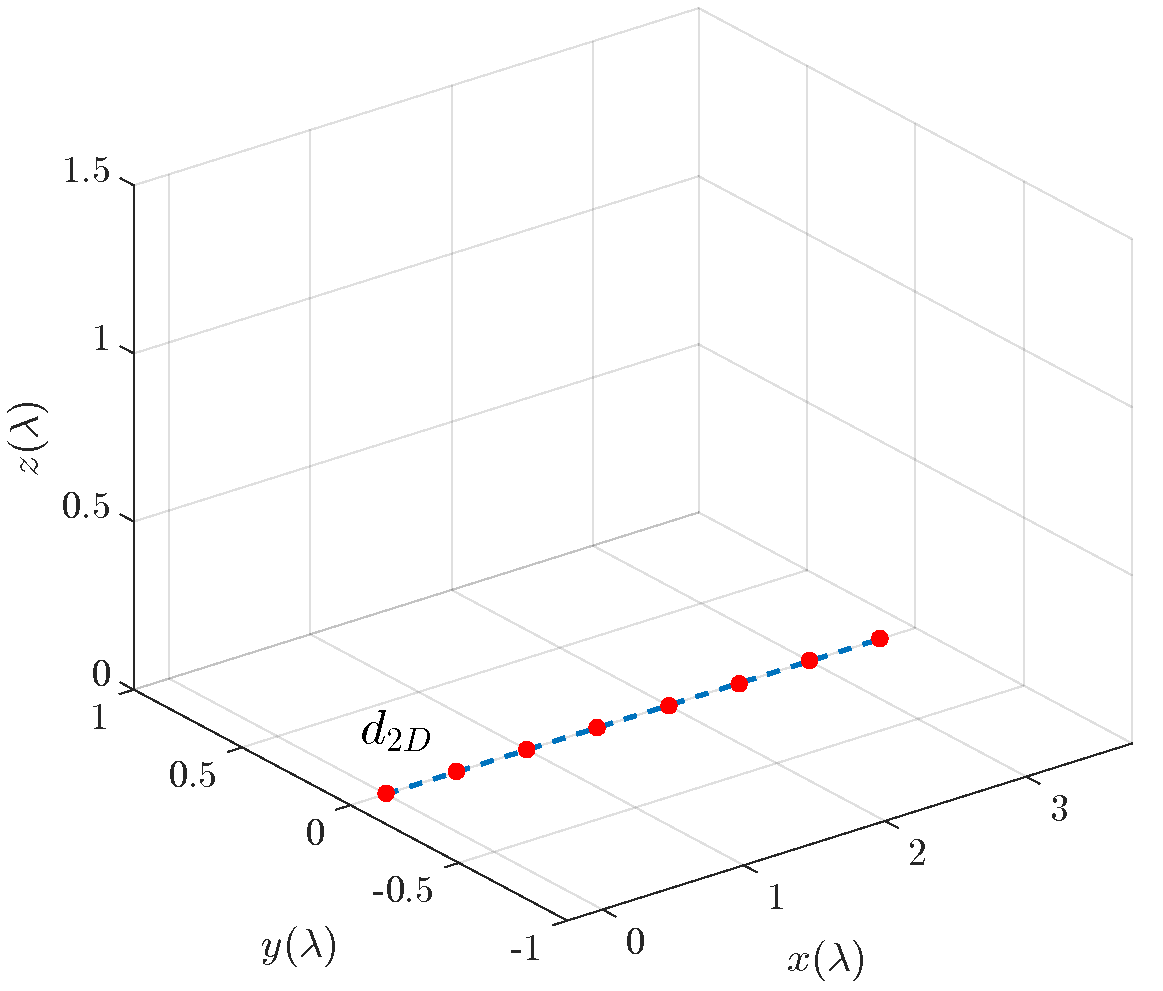
\includegraphics[width=\linewidth]{figures/ULA_2.pdf}}
    \hfill
    \subcaptionbox{Mảng trụ đồng nhất (UCyA - Uniform Cylindrical Array)}
        [0.49\linewidth]
        {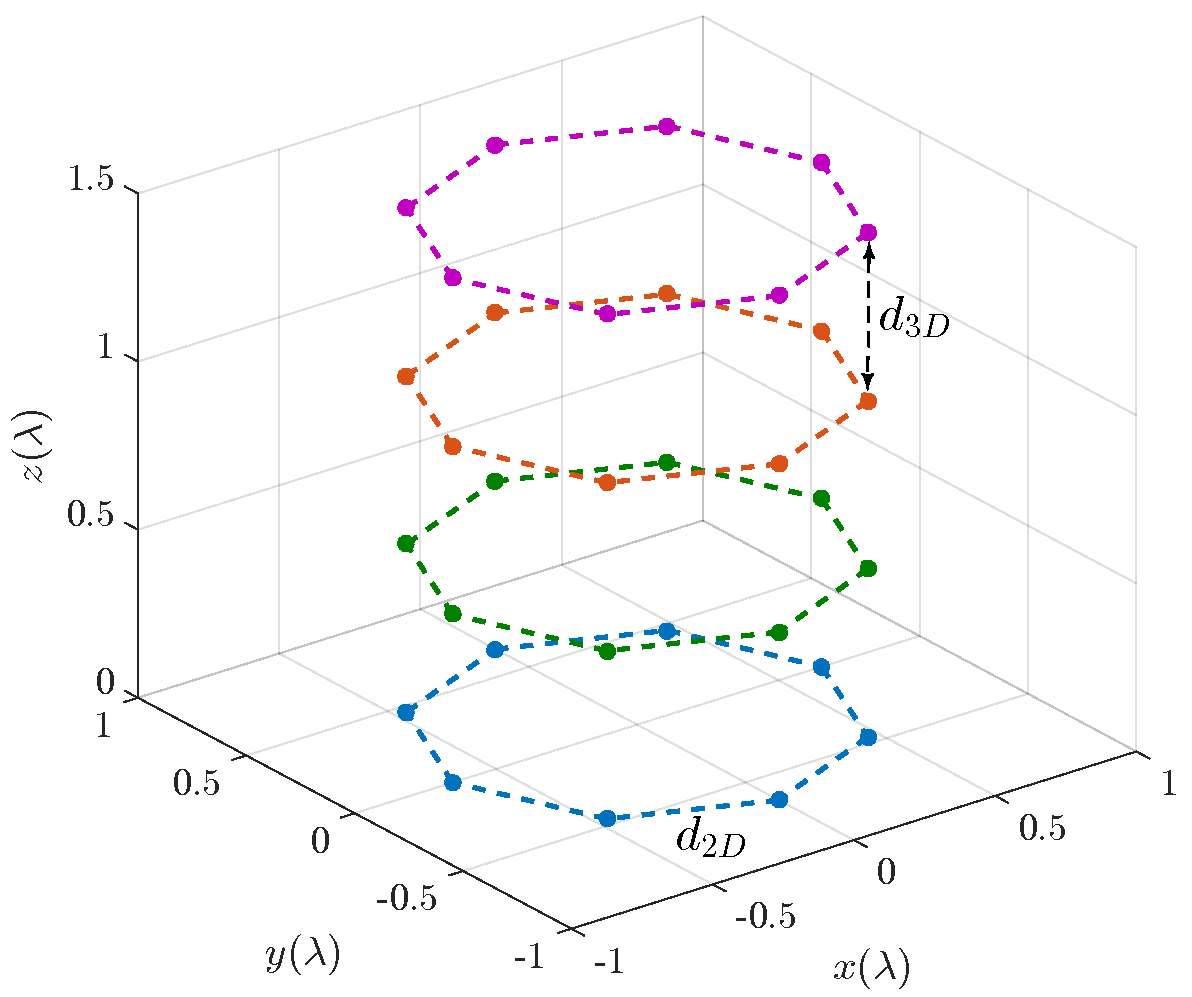
\includegraphics[width=\linewidth]{figures/UCyA_2.pdf}}
    \caption{Minh hoạ hai kiến trúc hình học 1D và 3D của các mảng ăng-ten.}
    \label{fig:antenstruct}
\end{figure}

Trong luận này, tác giả tập trung vào khảo sát hai cấu hình của các mảng ăng-ten được biểu diễn trên hình~\ref{fig:antenstruct} bao gồm mảng 1D và 3D~\cite{POORMOHAMMAD2017}. Ứng với mảng ăng-ten 1D, kiến trúc đơn giản nhất mảng thẳng cách đều (ULA) gồm $N_{ULA}$ phần tử được xem xét. Trong đó khoảng cách giữa các phần tử ăng-ten trong mảng ULA là $d_{2D}$. Ứng với mảng ăng-ten 3D, cấu hình mảng trụ đồng nhất (UCyA) gồm $N_{3D}$ lớp của $N_{UCA}$ phần tử thuộc mảng tròn cách đều (UCA - Uniform circle array) được xem xét. Với khoảng cách giữa các phần tử trong mảng UCA cũng là $d_{2D}$ và khoảng cách giữa các lớp của UCyA là $d_{3D}$ theo hướng của trục $z$. Từ đó, bán kính ($r$) của các mảng vòng UCA được tính như sau
% Particularly, we focus on two configurations of antenna arrays as shown in Fig.~\ref{fig:antenstruct}, i.e., 1D and 3D structures~\cite{POORMOHAMMAD2017}. For 1D arrays, we consider arrays with $N_{ULA}$~elements of ULA, where elements in these arrays are spaced by $d_{2D}$. For 3D arrays, UCyA consists of $N_{3D}$ layers of UCA (Uniform Circular Array) in size of $N_{UCA}$ elements. In this configuration, the spacing between two elements in UCA arrays is $d_{2D}$ and the distance between two layers is also $d_{3D}$ in $z$~direction. Thereby, the radius ($R$) of the UCA would be:
\begin{equation}
    r = \frac{1/2 \cdot d_{2D}}{\sin(\pi/N_{UCA})}
\end{equation}
% The position ($\boldsymbol{s}_p$) of each element in the array structures is expressed as follows:

Vị trí ($\boldsymbol{s}_p$) của các phần tử trong hai cấu hình mảng ăng-ten nêu trên là
\begin{align} 
    &\boldsymbol{s}_p(\text{ULA}) = \;\; \begin{cases}
    x_p = n_{ULA} \times d_{2D}\\ 
    y_p = 0\\ 
    z_p = 0
    \end{cases}
    % \\
    % &\boldsymbol{s}_p(\text{UCA}) = \;\; \begin{cases}
    % x_p = R \times \sin(n_{2D} \times \frac{2\pi}{N_{2D}})\\ 
    % y_p = R \times \cos(n_{2D} \times \frac{2\pi}{N_{2D}})\\ 
    % z_p = 0
    % \end{cases}
    \\
    &\boldsymbol{s}_p(\text{UCyA}) = \begin{cases}
    x_p = r \times \sin(n_{UCA} \times \frac{2\pi}{N_{UCA}})\\ 
    y_p = r \times \cos(n_{UCA} \times \frac{2\pi}{N_{UCA}})\\ 
    z_p = n_{3D} \times d_{3D}
    \end{cases}
\end{align}
với $n_{ULA} = 0, 1, \ldots, N_{ULA}-1$; $n_{UCA} = 0, 1, \ldots, N_{UCA}-1$, và $n_{3D} = 0, 1, \ldots, N_{3D}-1$.


\section{Cramér Rao Bound cho giải thuật nhận dạng hệ thống không mù và bán mù}\label{CRB}
% In this section, we present the CRB derivations for the unstructured channel model and specular channel model in both only pilots (OP) and semi-blind (SB) estimators for 3D-massive MIMO array geometries.
Trong mục này, tác giả sẽ trình bày về phương pháp đánh giá hiệu năng sử dụng đường CRB cho cả hai mô hình kênh truyền có cấu trúc (structured) và phi cấu trúc (unstructured) trong các hệ thống mMIMO. Sau đó, hai giải thuật ước lượng gồm chỉ sử dụng pilot (OP - Only pilot) và bán mù (SB) sử dụng thêm một phần thông tin từ đặc trưng thống kê của dữ liệu sẽ được so sánh độ chính xác cũng dựa trên đường CRB. 
\subsection{CRB trong trường hợp chỉ sử dụng pilot}

Như đã trình bày ở phần mở đầu của luận văn, việc sử dụng các ký hiệu pilot hay tín hiệu tham chiếu để ước lượng sử ảnh hưởng của kênh truyền vô tuyến là phương pháp mà WiFi hay 5G đang sử dụng. Về cơ bản, trong các bộ truyền phát sử dụng OFDM, $K_p$ ký hiệu pilot sẽ được chèn vào đoạn dữ liệu truyền đi và cả bên thu và phát đều biết trước các giá trị của các ký hiệu pilot này. Bên thu khai thác các ký hiệu pilot thu được để ước lượng ra sử ảnh hưởng của kênh truyền, từ đó nghịch đảo để khôi phục lại tín hiệu gốc. Tuy nhiên, không có cách nào có thể cho độ chính xác tuyệt đối trong việc nhận dạng kênh truyền vô tuyến thực. Do đó, các chuẩn truyền thông chỉ đưa ra phương pháp là tăng/giảm số lượng pilot khi kênh truyền ở các trạng thái khác nhau. Có một phương pháp được sử dụng rộng rãi để ước lượng độ chính xác tối đa của các bộ nhận dạng không thiên vị (unbias) đó là đường CRB~\cite{Kay1993}. Biểu diễn của CRB như sau

% Almost wireless communication standards use the training sequences in the physical layer (i.e., preamble) to estimate the effects of the propagation channel in the received signals. Typically, OFDM transceivers insert $K_p$ pilot symbols which are known in both the transmitter and receiver. Thus, the receiver can exploit these pilots for channel estimation. However, there is no way to perfect accuracy in wireless communication because we cannot compute a perfect CSI. To estimate the maximum possible accuracy in wireless communication systems, CRB is used for unbiased channel estimators. Basically, the CRB is given by~\cite{Kay1993}:
\begin{equation}
    \text{CRB}(\boldsymbol{\Theta}) = \mathbf{J}_{\boldsymbol{\Theta}\boldsymbol{\Theta}}^{-1}
\end{equation}
trong đó, $\mathbf{J}_{\boldsymbol{\Theta}\boldsymbol{\Theta}}$ là ma trận thông tin Fisher (FIM - Fisher information matrix) với $\boldsymbol{\Theta}$ là các véc-tơ tham số không biết trước cần được ước lượng. Trong mô hình kênh phi cấu trúc, $\boldsymbol{\Theta} \simeq	 \mathbf{h}$~\cite{Ladaycia2017}, FIM chỉ phụ thuộc vào các ký hiệu pilot nên sẽ được ký hiệu là $\mathbf{J}_{\boldsymbol{\Theta}\boldsymbol{\Theta}}^p$. Từ đó, các tham số cần được ước lượng sẽ được biểu diễn như sau~\cite{Menni2012}\footnote{Công suất nhiều được bỏ qua ($\sigma^2_{\mathbf{w}}$) do lỗi ước lượng của tạp âm không ảnh hưởng đến $\mathbf{h}$.}:
\begin{equation}
    \boldsymbol{\Theta}=\left[\boldsymbol{\Psi}^{\top},  \quad  \left(\boldsymbol{\Psi}^{*}\right)^{\top}\right]
\end{equation}

Trong các hệ thống mMIMO-OFDM, $K_p$ ký hiệu pilot sẽ được sắp xếp trong các ký hiệu OFDM~\cite{Garro2020} và do giả thiết tạp âm là một quá trình ngẫu nhiên i.i.d. FIM trong trường hợp chỉ sử dụng pilot (OP) thu được như sau
% In MIMO-OFDM systems, $K_p$ pilots are arranged in OFDM symbols~\cite{Garro2020}, and since the noise is an i.i.d random process, we could formulate FIM in only pilots (OP) case as follows:
\begin{equation}
\label{eq:9}
    \mathbf{J}_{\boldsymbol{\Theta} \boldsymbol{\Theta}}^{p}=\sum_{i=1}^{K_{p}} \mathbf{J}_{\boldsymbol{\Theta} \boldsymbol{\Theta}}^{p_{i}}
\end{equation}
với $\mathbf{J}_{\boldsymbol{\Theta} \boldsymbol{\Theta}}^{p_{i}}$ là FIM tương ứng với pilot thứ $i$~\cite{Kay1993} được cho bởi
\begin{equation}
    \label{eq:10}
    \begin{aligned}
        \mathbf{J}_{\boldsymbol{\Theta} \boldsymbol{\Theta}}^{p_{i}} &=\mathbb{E}\left\{\left(\frac{\partial \ln p(\mathbf{x}(i), \boldsymbol{\Psi})}{\partial \boldsymbol{\Theta}^{*}}\right)\left(\frac{\partial \ln p(\mathbf{x}(i), \boldsymbol{\Psi})}{\partial \boldsymbol{\Theta}^{*}}\right)^{H}\right\} \\
        % &=\left(\begin{array}{cc}
        % \mathbf{J}_{\boldsymbol{\Psi} \boldsymbol{\Psi}}^{p_{i}} & \mathbf{0} \\
        % \mathbf{0} & \mathbf{J}_{\boldsymbol{\Psi}^{*} \boldsymbol{\Psi}^{*}}^{p_{i}}
        % \end{array}\right)
    \end{aligned}
\end{equation}
trong đó $\mathbb{E}$ là toán tử kỳ vọng; $p(\mathbf{x}(i), \boldsymbol{\Psi})$ là hàm mật độ xác suất (Pdf - Probability density function) của tín hiệu nhận được đã biết $\boldsymbol{\Psi}$. Phương trình~(\ref{eq:10}) gồm các phép đạo hàm số phức, nên có thể biểu diễn dưới dạng
\begin{equation}
    \mathbf{J}_{\boldsymbol{\theta} \mathbf{\theta}}^{p_{i}}=\frac{\mathbf{s}(i)^{H} \mathbf{s}(i)}{\sigma_{\mathbf{w}}^{2}}
\end{equation}

Tiếp đến, mô hình kênh có cấu trúc như trên phương trình~(\ref{eq:2}) được xem xét. Véc-tơ tham số có kích thước $4T~\times M$ cần được ước lượng là

% When considering a structured model for channel impulse response as shown in~(\ref{eq:2}), the parameters vector of size \mbox{$4N_t~\times L$} to be estimated is given by:
\begin{equation}
    \boldsymbol{\Theta}=\left[ \boldsymbol{\beta}^\top, \quad \boldsymbol{(\beta^*)}^\top, \quad \boldsymbol{\theta}^\top, \quad \boldsymbol{\phi}^\top \right]
\end{equation}
với $\boldsymbol{\beta}=\left[\beta_{0,0}, \ldots, \beta_{M-1, T -1}\right]^{\top}$, $\boldsymbol{\beta^*}=\left[\beta^*_{0,0}, \ldots, \beta^*_{M-1, T - 1}\right]^{\top}$, $\boldsymbol{\theta}=\left[\theta_{0,0}, \ldots, \theta_{M-1, T - 1}\right]^{\top}$, và $\boldsymbol{\phi}=\left[\phi_{0,0}, \ldots, \phi_{M-1, T - 1}\right]^{\top}$ lần lượt tương ứng là các véc-tơ có kích thước $T \times M$ của hệ số khuếch đại phức, liên hợp phức của hệ số khuếch đại phức, góc ngẩng, và góc phương vị của DoA. Dựa trên phép chuyển đổi của việc đạo hàm theo các tham số kể trên, FIM ($\mathbf{J}^p_{\mathbf{h} \mathbf{h}}$) của kênh truyền $\mathbf{h}$ trên (\ref{eq:1}) sẽ là
% with the complex gain, the conjugate of complex gain, zenith, and azimuth angle of DoA vectors of size $T \times M$ respectively are $\boldsymbol{\beta}=\left[\beta_{0,0}, \ldots, \beta_{M-1, T -1}\right]^{\top}$, $\boldsymbol{\beta^*}=\left[\beta^*_{0,0}, \ldots, \beta^*_{M-1, T - 1}\right]^{\top}$, $\boldsymbol{\theta}=\left[\theta_{0,0}, \ldots, \theta_{M-1, T - 1}\right]^{\top}$, and $\boldsymbol{\phi}=\left[\phi_{0,0}, \ldots, \phi_{M-1, T - 1}\right]^{\top}$. Regarding to the FIM derivation of parameters transformation~\cite{Kay1993}, the FIM ($\mathbf{J}^p_{\mathbf{h} \mathbf{h}}$) of channel $\mathbf{h}$ in (\ref{eq:1}) would be:

\begin{equation}
\label{eq:13}
    \mathbf{J}^p_{\mathbf{h} \mathbf{h}}=\frac{\partial \mathbf{h}}{\partial \boldsymbol{\Theta}} \mathbf{J}^p_{\Theta \Theta} {\frac{\partial \mathbf{h}}{\partial \boldsymbol{\Theta}}}^{H}
\end{equation}
với 
\begin{equation}
\label{eq:2.15}
    \frac{\partial \mathbf{h}}{\partial \boldsymbol{\Theta}}=
    \left[\frac{\partial \mathbf{h}}{\partial \boldsymbol{\beta}}, 
    \frac{\partial \mathbf{h}}{\partial \boldsymbol{\beta^*}},
    \frac{\partial \mathbf{h}}{\partial \boldsymbol{\theta}}, 
    \frac{\partial \mathbf{h}}{\partial \boldsymbol{\phi}}\right]
\end{equation}
% More particularly, we express the derivations as follows:
Chi tiết hơn, ví dụ đạo hàm riêng theo $\boldsymbol{\beta}$ trên phương trình~(\ref{eq:2.15}) có dạng như sau
\begin{subequations}
    \begin{align}
    &\frac{\partial \mathbf{h}}{\partial \boldsymbol{\beta}}=
    \left[\begin{array}{llll}
        \boldsymbol{B}_{0}^{\top}, & \boldsymbol{B}_{1}^{\top}, & \ldots, & \boldsymbol{B}_{L - 1}^{\top}
    \end{array}\right]^{\top}\\
    &\boldsymbol{B}_{l}=\operatorname{diag}\left(\left[\boldsymbol{B}_{l, 0}, \quad \boldsymbol{B}_{l, 1}, \quad \ldots, \quad \boldsymbol{B}_{l, T - 1}\right]\right) \\
    &\boldsymbol{B}_{l, t}=\left[\begin{array}{cccc}
        \frac{\partial h_{l, t}}{\partial \beta_{0, t}} &
        \frac{\partial h_{l, t}}{\partial \beta_{1, t}} & 
        \ldots & 
        \frac{\partial h_{l, t}}{\partial \beta_{M-1, t}}
    \end{array}\right]^\top
    \end{align}
\end{subequations}
Các đạo hàm riêng của $\boldsymbol{B}_{l,t}$ được biểu diễn chi tiết trên các phương trình (\ref{eq:15}).

% \begin{figure}[!b]
    % \hrule
    % \vspace{0.5cm}

\begin{subequations}
\label{eq:15}
    \begin{align}
    &\frac{\partial h_{l, t}}{\partial \beta_{m, t}}= \frac{1}{2} (1 - i) \cdot e^{-i k_s c(\theta_{m, t}, \phi_{m, t})} &  \\
    &\frac{\partial h_{r, j}}{\partial \beta^*_{m, t}}= \frac{1}{2} (1 + i) \cdot e^{-i k_s c(\theta_{m, t}, \phi_{m, t})} \\
    &\frac{\partial h_{l, t}}{\partial \theta_{m, t}}=
    \beta_{m, t} 
    [-i k_s (\cos\theta_{m, t} \cos\phi_{m, t} x_p + \cos\theta_{m, t} \sin\phi_{m, t} y_p
    - \sin \theta_{m, t} z_p)] \cdot e^{-j k_s c(\theta_{m, t}, \phi_{m, t})} \\ 
    &
    \resizebox{\textwidth}{!}{$\frac{\partial h_{l, t}}{\partial \phi_{m, t}}=\beta_{m, t}
     [-i k_s (-\sin\theta_{m, t} \sin\phi_{m, t} x_p + \sin\theta_{m, t} \cos\phi_{m, t} \cdot y_p 
    + \cos \theta_{m, t} z_p)] \cdot e^{-i k_s c(\theta_{m, t}, \phi_{m, t})}$ 
    }
    \end{align}
\end{subequations}
% \end{figure}

\subsection{CRB trong trường hợp bán mù}

Theo hướng tiếp cận SB, ngoài sử dụng các ký hiệu pilot, các bộ nhận dạng còn sử dụng thêm thông tin từ các ký hiệu dữ liệu không biết trước trong việc ước lượng kênh truyền. Trong phần này, học viên giả thiết các ký hiệu pilot và dữ liệu trong các ký hiệu OFDM là độc lập về mặt thống kê. Từ đó, FIM của phương pháp SB này có thể được biểu diễn đơn giản là tổng của FIM từ các ký hiệu pilot và FIM từ các ký hiệu data như dưới đây

% In the SB approach, besides using pilots, estimators also use other information of the unknown data to aid in channel estimation. In this paper, we supposed that pilots and data in OFDM symbols are statistically independent. So, the FIM of this strategy is formulated as follows:
\begin{equation}
    \label{eq:17}
    \mathbf{J}_{\boldsymbol{\Theta} \boldsymbol{\Theta}}^{SB}= \mathbf{J}_{\boldsymbol{\Theta} \boldsymbol{\Theta}}^{p} + \mathbf{J}_{\boldsymbol{\Theta} \boldsymbol{\Theta}}^{d}
\end{equation}
với $\mathbf{J}_{\boldsymbol{\Theta} \boldsymbol{\Theta}}^{d}$ tương ứng là FIM của các ký hiệu data chưa biết trước và $\mathbf{J}_{\boldsymbol{\Theta} \boldsymbol{\Theta}}^{p}$ FIM của các ký hiệu pilot như đã được trình bày trên phương trình~(\ref{eq:9}). Giả sử $K_d$ ký hiệu data là i.i.d với trung bình thống kê là $0$ và thông tin SOS là ma trận hiệp phương sai $\mathbf{C}_{\mathbf{s}}=\operatorname{diag}\left(\boldsymbol{\sigma}_{\mathbf{s}}^{2}\right)$. Trong đó, $\boldsymbol{\sigma}_{\mathbf{s}}^{2} \stackrel{\operatorname{def}}{=}\left[\sigma_{\mathbf{s}_{0}}^{2}, \ldots, \sigma_{\mathbf{s}_{T-1}}^{2}\right]^\top$ với $\sigma_{\mathbf{s}_t^{2}}$ là công suất truyền tại ăng-ten thứ $t$. Ma trận hiệp phương sai $\mathbf{C}_{\mathbf{x}}$ là:
\begin{equation}
    \mathbf{C}_{\mathbf{x}}=\sum_{t=0}^{T-1} \sigma_{\mathbf{s}_{t}}^{2} \boldsymbol{\lambda}_{t} \boldsymbol{\lambda}_{t}^{H}+\sigma_{\mathbf{w}}^{2} \mathbf{I}_{K L}
\end{equation}
trong đó, $\mathbf{I}_{KL}$ là ma trận đơn vị có kích thước $K L$ và $\boldsymbol{\lambda}$ được định nghĩa là:
\begin{equation}
    \begin{aligned}
        \boldsymbol{\lambda} &=\left[\boldsymbol{\lambda}_{0}, \boldsymbol{\lambda}_{1}, \ldots, \boldsymbol{\lambda}_{T-1}\right] \\ 
        \boldsymbol{\lambda}_{t}&=\left[\boldsymbol{\lambda}_{0, t}, \boldsymbol{\lambda}_{1, t}, \ldots, \boldsymbol{\lambda}_{L-1, t}\right]^{\top}
    \end{aligned}
\end{equation}
với $\boldsymbol{\lambda}_{l, t}=\operatorname{diag}\left(\mathcal{F}_0 h_{l, t}\right)$ trong đó, $\mathcal{F}_0$ là cột đầu tiên của ma trận $\mathcal{F}$. FIM của các ký hiệu data có dạng như sau:
\begin{equation}
    \mathbf{J}_{\boldsymbol{\Theta} \boldsymbol{\Theta}}^{d}=K_{d}\left[\begin{array}{cc}
    \mathbf{J}_{\boldsymbol{\Psi} \boldsymbol{\Psi}}^{d} & \mathbf{J}_{\boldsymbol{\Psi} \boldsymbol{\Psi}^{*}}^{d} \\
    \mathbf{J}_{\boldsymbol{\Psi}^{\star} \boldsymbol{\Psi}}^{d} & \mathbf{J}_{\boldsymbol{\Psi}^{\star} \boldsymbol{\Psi}^{*}}^{d}
    \end{array}\right]
\end{equation}

Theo~\cite{Kay1993}, FIM $\mathbf{J}_{\boldsymbol{\Theta} \boldsymbol{\Theta}}^{d}$ của các ký hiệu data sẽ được biến đổi về dạng cuối cùng là
\begin{equation}
    \mathbf{J}_{\boldsymbol{\Theta} \boldsymbol{\Theta}}^{d}=\operatorname{tr}\left\{\mathbf{C}_{\mathbf{x}}^{-1} \frac{\partial \mathbf{C}_{\mathbf{x}}}{\partial \boldsymbol{\Psi}^{*}} \mathbf{C}_{\mathbf{x}}^{-1}\left(\frac{\partial \mathbf{C}_{\mathbf{x}}}{\partial \boldsymbol{\Psi}^{*}}\right)^{H}\right\}
\end{equation}
trong đó, $\frac{\partial \mathbf{C}_{\mathbf{x}}}{\partial \mathbf{h}_{t}^{*}}=\boldsymbol{\lambda} \mathbf{C}_{\mathbf{s}} \frac{\partial \boldsymbol{\lambda}^{H}}{\partial \mathbf{h}_{t}^{*}}$ và $\operatorname{tr}$ là toán tử tính tổng các thành phần trên đường chéo của một ma trận. Nếu sử dụng mô hình kênh phi cấu trúc, CRB của phương pháp SB sẽ là nghịch đảo của phương trình (\ref{eq:17}). Ngược lại, nếu sử dụng mô hình kênh có cấu trúc, CRB của phương pháp SB thu được bằng cách đưa FIM ở phương trình (\ref{eq:17}) qua phép chuyển đổi đã trình bày tại phương trình (\ref{eq:13}).
% In the unstructured channel model approach, the CRB of the SB method is the inverse of (\ref{eq:17}). Similar to the OP method, the CRB of the SB method using the specular channel model is given by applying (\ref{eq:17}) to the transformation in (\ref{eq:13}).

\section{Mô phỏng và đánh giá}\label{SR}

% ~\cite{Raghavan2017} ~\cite{Ko2017} ~\cite{Ju2021}
Để xem xét ảnh hưởng của cấu hình mảng ăng-ten trong hệ thống mMIMO, ba kịch bản mô phỏng sẽ được xem xét. Cụ thể, tác giả ước lượng đường CRB của việc ước lượng kênh truyền khi: (i) SNR thay đổi; (ii) số lượng các lớp $N_{3D}$ của kiến trúc UCyA thay đổi; (iii) số lượng phần tử $N_{UCA}$ của mảng tròn UCA thay đổi. Các thông số mô phỏng của hệ thống truyền thông MIMO kích thước lớn được sử dụng có tại bảng~\ref{tab:simulation_param_CRB}~\cite{Swindlehurst2022}. Các kết quả mô phỏng được lấy trung bình của $1.000$ lần chạy và các đường CRB được chuẩn hoá dưới dạng $\log_{10} (\operatorname{CRB})$.
% In this section, we simulate three scenarios to verify the performance of SB and UCyA antenna structures. In detail, there are channel estimation CRBs versus, i.e., SNR (signal noise ratio), the number of UCyA layers $N_{3D}$, and the number of UCA elements $N_{UCA}$. The simulation parameters of a massive MIMO system are shown in Table~\ref{tab:simulation_param_CRB}~\cite{Swindlehurst2022}. The simulation results are obtained by average of 1,000 running times.
\begin{table}[ht]
\centering
\caption{Các tham số mô phỏng hệ thống truyền thông không dây để ước lượng CRB.}
\label{tab:simulation_param_CRB}
\begin{tabular}{p{8cm} | p{6cm}}
\hline
\hline
\multicolumn{1}{c|}{\textbf{Thông số mô phỏng}} & \multicolumn{1}{c}{\textbf{Giá trị}} \\ \hline
Kích thước hệ thống mMIMO                            & $T = 2$      \\ \hline
Khoảng cách giữa các phần tử ăng-ten                 & $d_{2D} = d_{3D} = \lambda / 2$ \\ \hline
Số lượng các đường truyền                   & $M = 4$      \\ \hline
Số sub-carriers                    & $K = 64$     \\ \hline
Số Pilot, Data symbols                          & $K_p = 16, K_d = 48$     \\ \hline
Hệ số khuếch đại phức               & $\beta \sim \mathcal{C} \mathcal{N}\left(0, 1 \right)$     \\ \hline
Góc phương vị của DoA            & $\phi^\circ \sim \mathcal{U}(-\pi/2, \pi/2)$        \\ \hline
Góc ngẩng của DoA           & $\theta^\circ \sim \mathcal{U}(-\pi/2, \pi/2)$       \\ \hline
\end{tabular}
\end{table}
\begin{figure}[!b]
    \centering
    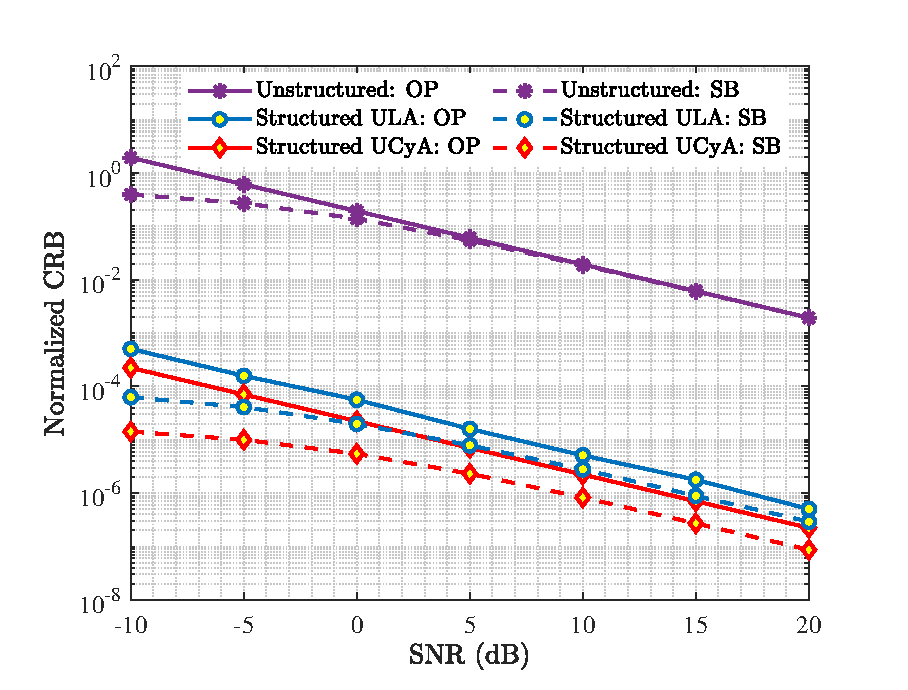
\includegraphics[width=\linewidth]{figures/fig_1_3.eps}
    \caption{CRB của hai kiến trúc ULA và UCyA ứng với mô hình kênh truyền có cấu trúc (structured) và phi cấu trúc (unstuctured). Cấu hình của mảng ăng-ten như sau $N_{ULA} = 96, N_{UCA} = 24,$ và $N_{3D} = 4$.}
    \label{fig:op}
\end{figure}

Trên hình~\ref{fig:op}, số lượng phần tử của mảng thu MIMO kích thước lớn là $96$ trong đó $N_{ULA}~=~96, N_{UCA} = 24,$ và $N_{3D} = 4$. Nhìn chung, sai số ước lượng của mô hình kênh truyền có cấu trúc vượt trội rõ ràng khi so sánh với mô hình kênh truyền phi cấu trúc với độ lợi khoảng $10^3$~dB. Khi so sánh về hai phương pháp ước lượng SB và OP, ở các mức SNR thấp (SNR $\le$ $5$~dB), phương pháp SB áp dụng cho mô hình kênh truyền phi cấu trúc có thể cho sai số thấp hơn một chút khi so sánh với việc chỉ sử dụng pilot của OP. Với mô hình kênh structured, phương pháp SB vẫn cho CRB tốt hơn ở các mức SNR thấp, và giữ ở mức ổn định khi SNR $\ge 5$~dB. Tiếp đến là so sánh về ảnh hưởng của cấu hình mảng ăng-ten, cấu hình UCyA cho độ chính xác cao hơn so với ULA ở cả hai phương pháp ước lượng OP và SB. Có thể rút ra nhận xét, việc sử dụng mô hình kênh truyền có cấu trúc, phương pháp ước lượng SB, và cấu hình mảng ăng-ten 3D (UCyA) có thể cho ra độ chính xác cao hơn cho các bộ nhận dạng của hệ thống mMIMO.
% In Fig.~\ref{fig:op}, the number of massive MIMO antennas is 96 where $N_{ULA} = 96, N_{UCA} = 24, N_{3D} = 4$. Overall, CRBs of the specular channel model approach clearly outperform those of the unstructured at $10^3$~dB of gain. At lower SNR values (SNR $\le 5$~dB), the unstructured CRB of SB method is slightly better than the only pilot one. In the specular approach, the difference between the CRB of pilots and SB methods is evident at SNR values lower than $5$~dB and remains stable at higher SNR values. While massive MIMO array geometries show that the CRB of UCyA structure is also higher accurate than that of ULA structure in both pilots and SB method. Thus, it can be shown that the use of specular models, SB estimation methods, and 3D antenna arrays can provide higher performance for channel estimators in massive MIMO systems.
\begin{figure}[H]
    \centering
    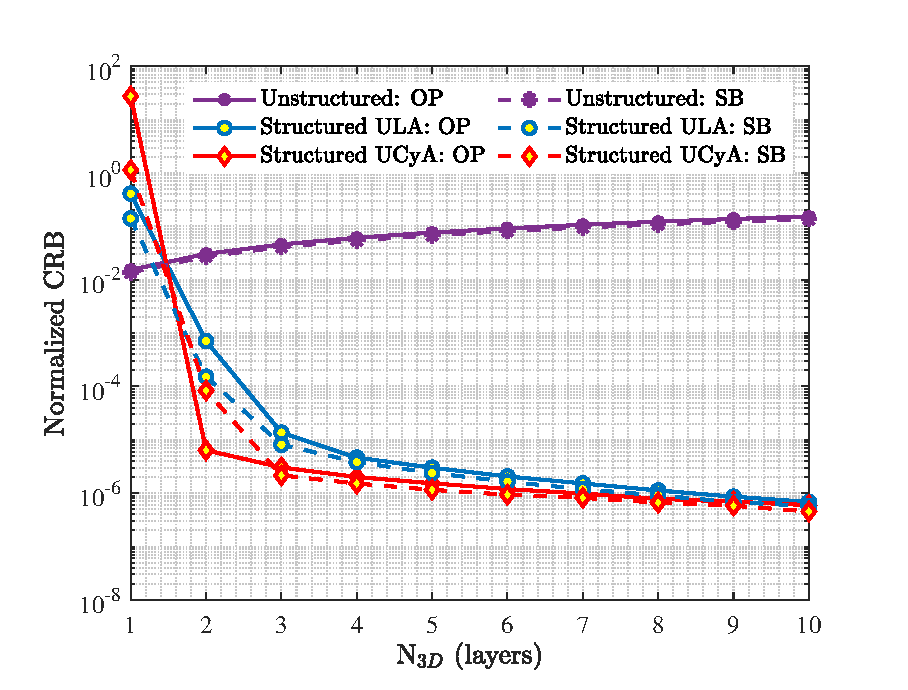
\includegraphics[width=\linewidth]{figures/fig_2_3.eps}
    \caption{CRB của hai kiến trúc ULA và UCyA khi thay đổi $N_{3D}$. Các thông số mô phỏng như sau $N_{UCA} = 24, N_{ULA} = 24 \times N_{3D}$, và SNR $=5$~dB.}
    \label{fig:op_N3D}
\end{figure}

Trên hình~\ref{fig:op_N3D}, số lượng các lớp $N_{3D}$ của kiến trúc UCyA được khảo sát bằng cách giữ nguyên số phần tử thuộc mảng vòng $N_{UCA} = 24$ và SNR~$=5$~dB. Một lần nữa, các đường CRB chỉ ra rằng với $N_{3D}$ khác nhau mô hình kênh truyền có cấu trúc hầu như có thể cho ra độ chính xác cao hơn mô hình kênh truyền phi cấu trúc. Xét riêng mô hình kênh truyền unstructured, số $N_{3D}$ tăng lên kéo theo sai số ước lượng cũng tăng lên dù không quá lớn. Ngay cả khi sử dụng phương pháp ước lượng SB, độ chính xác thu được với unstructured gần như không được cải thiện. Ngược lại, với mô hình kênh truyền structured, đường CRB có xu hướng đi xuống khi số lớp của mảng UCyA tăng cho đến khi tất cả hội tụ tại sai số khoảng $10^{-6}$. Tại các giá trị $N_{3D}$ nhỏ, trong khoảng từ $2$ đến $6$ lớp, việc sử dụng kiến trúc UCyA nhìn chung vẫn cho hiệu quả đáng kể so với ULA. Khi xem xét sự ảnh hưởng của phương pháp OP hay SB trong kịch bản này, rõ ràng không có sự khác biệt quá rõ ràng nếu $N_{3D} \ge 3$. Có thể rút ra nhận xét thứ hai, sử dụng mô hình kênh truyền có cấu trúc và cấu hình mảng UCyA có thể cho hiệu suất ước lượng kênh truyền tốt hơn khi $N_{3D}$ nhỏ. Tuy nhiên, lưu ý rằng, ngoài lợi thế về độ chính xác, khi số lượng phần tử trong mảng lên đến $240$ như trong mô phỏng, cấu hình mảng UCyA sẽ giúp tiết kiệm được rất nhiều diện tích lắp đặt mảng ăng-ten.
% In Fig.~\ref{fig:op_N3D}, the number of layers $N_{3D}$ in the UCyA structures is investigated by fixing $N_{UCA}$ elements at 24 and SNR $=5$~dB. Again, the CRBs of the specular channel model give superior quality to those of the unstructured model. The first point, when the number of antennas increases, the CRB of the unstructured model also increases. Moreover, the SB channel estimation method in this case is also almost trivial. On the other hand, CRBs in the specular approach tend to decrease as the number of antennas increases until all of them converge to a point at $10^{-6}$. At $N_{3D}$ values as low as 2 to 6 layers, the UCyA structure still gives a relatively significant quality when compared to the ULA in both NB and SB methods. Hence, the specular model method gives a better channel estimation error rate while 3D antenna arrays are valuable when the number of layers is small. However, note that, in addition to the advantage of accuracy in channel estimation, UCyA structures save powerful deployment areas.

Cuối cùng, trên hình~\ref{fig:op_NUCA}, số lượng phần tử của mảng tròn UCA được thay đổi trong khoảng từ $8$ đến $64$ phần tử, trong khi giữ nguyên $N_{3D} = 4, N_{ULA} = 4 \times N_{UCA}$, và SNR $=5$~dB. Do CRB của mô hình kênh truyền phi cấu trúc chỉ bị ảnh hưởng bởi số lượng phần tử ăng-ten nên các đường CRB vẫn giữ như trên hình~\ref{fig:op_N3D}. Với mô hình kênh truyền có cấu trúc, CRB thay vì hội tụ tại một điểm sẽ có xu hướng giảm dần cùng với $N_{UCA}$. Khi số phần tử $N_{UCA}$ đủ lớn ($N_{UCA} \ge 24$), các đường CRB của UCyA cho độ chính xác tốt hơn một cách tuyến tính khi so sánh với mảng ULA. Phương pháp SB trong kịch bản mô phỏng này nhìn chung chỉ cho độ chính xác tốt hơn nhưng không nhiều so với OP. Có thể rút ra nhận xét thứ ba, sử dụng mô hình kênh truyền có cấu trúc và cấu hình mảng UCyA có thể cho hiệu suất ước lượng kênh truyền tốt hơn và tăng dần với $N_{UCA}$. Tuy nhiên, cần lưu ý dù cho độ chính xác cao hơn, nhưng khi $N_{UCA}$ tăng cao, bán kính của mảng tròn UCA lớn dần lại dẫn đến lãng phí diện tích lắp đặt mảng ăng-ten.
% At last, in Fig.~\ref{fig:op_NUCA} the number of UCA elements $N_{UCA}$ is turn in range 8 to 64 elements while $N_{3D} = 4, N_{ULA} = 4 * N_{UCA}$, and SNR $=5$~dB. Since the unstructured performance is only affected by the number of antennas, its performance remains at the same levels as shown in Fig.~\ref{fig:op_N3D}. However, instead of converging as before in Fig.~\ref{fig:op_N3D}, the CRBs in the specular approach gradually reduce as $N_{UCA}$ continues to rise. At large $N_{UCA}$ elements, UCyA arrays linearly give better performance than ULA arrays. Note that, despite the accuracy benefits, it is more complicated to produce large UCA arrays.
\begin{figure}[ht]
    \centering
    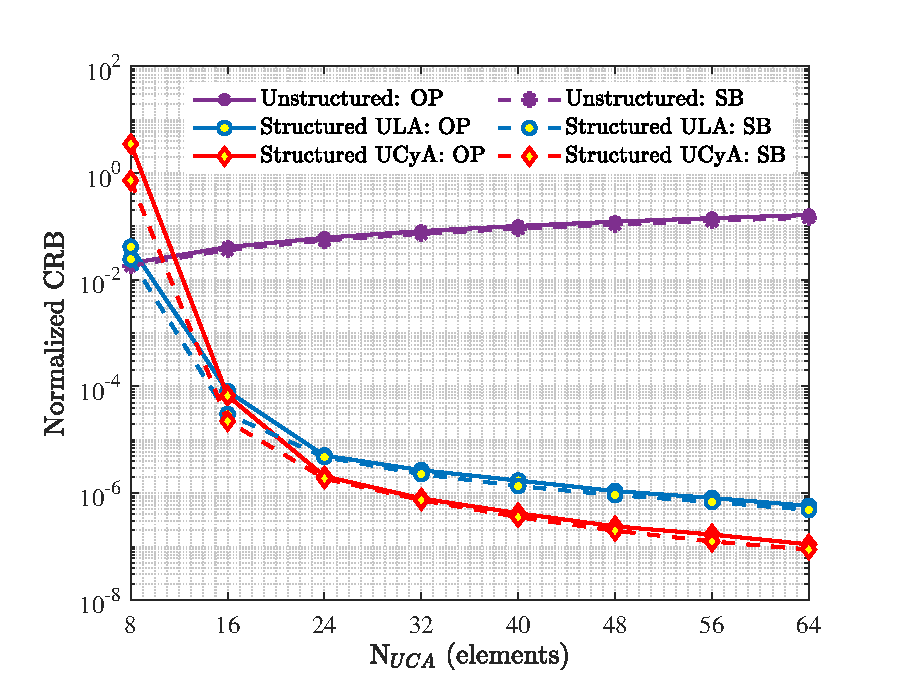
\includegraphics[width=\linewidth]{figures/fig_3_3.eps}
    \caption{CRB của hai kiến trúc ULA và UCyA khi thay đổi $N_{UCA}$. Các thông số mô phỏng như sau $N_{3D} = 4, N_{ULA} = 4 \times N_{UCA}$, và SNR $=5$~dB.}
    \label{fig:op_NUCA}
\end{figure}

\section{Kết luận chương}
% In this paper, Cramér Rao Bound is used to analyze the effect of antenna array geometry on channel estimation errors in massive MIMO-OFDM systems. The CRBs of channel estimation in both cases, i.e., only pilot and semi-blind based methods, are presented. The simulation results demonstrate that the performance of the system is significantly improved in the structured channel model. In this model, the UCyA structure obtains fewer channel estimation errors, and this geometry is more suitable than the traditional ULA structure.
Trong chương này, Cramér Rao Bound đã được sử dụng để xem xét hiệu quả của các cấu hình mảng ăng-ten khác nhau đến sai số ước lượng kênh truyền trong các hệ thống mMIMO. Lý thuyết về đường CRB cho việc ước lượng kênh truyền được trình bày trong hai trường hợp OP và một phương pháp SB. Các kết quả mô phỏng đã chỉ ra hiệu năng của việc ước lượng kênh truyền có thể được cải thiện rõ rệt nếu sử dụng mô hình kênh truyền có cấu trúc. Ngoài ra, cấu hình mảng ăng-ten UCyA và phương pháp SB cũng sẽ góp phần cải thiện độ chính xác khi so sánh với kiến trúc ULA và phương pháp OP truyền thống.